\documentclass[11pt,a4paper]{article}
\usepackage[margin=18mm,top=22mm,bottom=18mm,headsep=7mm,footskip=9mm]{geometry}
\usepackage{fontspec,amsmath,amssymb,array,tabularx,xcolor,colortbl,tikz,fancyhdr,hyperref,graphicx}
\setmainfont{NotoSansKR-Regular.ttf}[Path=../../../common/assets/fonts/,BoldFont=NotoSansKR-Semibold.ttf]
\newfontfamily\brandfont{NotoSansKR-Regular.ttf}[Path=../../../common/assets/fonts/,BoldFont=NotoSansKR-Semibold.ttf]
\XeTeXlinebreaklocale "ko"
\XeTeXlinebreakskip=0pt plus 1pt
\definecolor{ink}{HTML}{25343D}
\definecolor{blue}{HTML}{216B7A}
\definecolor{grid}{HTML}{CED7DB}
\definecolor{soft}{HTML}{F2F6F6}
\definecolor{body}{HTML}{303D44}
\definecolor{muted}{HTML}{637078}
\hypersetup{colorlinks=true,urlcolor=blue,pdftitle={OZ Lab - AI Study, Cost Function / Gradient Descent},pdfauthor={OZ Lab}}
\setlength{\parindent}{0pt}
\setlength{\parskip}{2pt}
\setlength{\headheight}{21pt}
\setlength{\tabcolsep}{6pt}
\renewcommand{\arraystretch}{1.3}
\arrayrulecolor{grid}
\pagestyle{fancy}\fancyhf{}
\fancyhead[L]{\brandfont\fontsize{8}{10}\selectfont\bfseries\color{ink} OZ Lab - AI Study}
\fancyhead[R]{\brandfont\fontsize{7.5}{10}\selectfont\color{muted} Cost Function / Gradient Descent}
\fancyfoot[L]{\brandfont\fontsize{7}{9}\selectfont\color{muted} MACHINE LEARNING\quad /\quad C1 W1}
\fancyfoot[R]{\brandfont\fontsize{8}{10}\selectfont\color{ink}\ifnum\value{page}<10 0\fi\thepage\quad{\color{muted}/\ 06}}
\renewcommand{\headrulewidth}{.3pt}
\renewcommand{\headrule}{\hbox to\headwidth{\color{grid}\leaders\hrule height\headrulewidth\hfill}}
\newcommand{\titleline}[3]{\par\noindent\makebox[10mm][l]{\brandfont\fontsize{11}{16}\selectfont\bfseries\color{blue}#1}{\fontsize{15}{20}\selectfont\textcolor{ink}{\textbf{#2}}}\par\if\relax\detokenize{#3}\relax\else\vspace{1mm}\hspace*{10mm}{\fontsize{8}{12}\selectfont\color{muted}#3}\par\fi\vspace{5mm}}
\newcommand{\q}[2]{\par\vspace{3.5mm}\noindent\makebox[7mm][l]{\brandfont\fontsize{8.5}{13}\selectfont\bfseries\color{blue}#1}\begin{minipage}[t]{\dimexpr\linewidth-7mm}\fontsize{9.3}{14}\selectfont #2\end{minipage}\par}
\newcommand{\blank}[1]{{\color{muted}\rule{#1}{.3pt}}}
\newcommand{\lines}[1]{\par\foreach \n in {1,...,#1}{\vspace{8mm}\par\hspace*{7mm}{\color{grid}\rule{\dimexpr\linewidth-7mm}{.3pt}}}\par}
\newcommand{\note}[1]{\par\vspace{.6mm}\noindent\hspace*{7mm}\begin{minipage}{\dimexpr\linewidth-7mm}\fontsize{7.8}{11.5}\selectfont\color{muted}* #1\end{minipage}\par}
\newcommand{\formula}[1]{\par\vspace{1.5mm}\noindent\hspace*{7mm}\begingroup\setlength{\fboxsep}{3mm}\colorbox{soft}{\begin{minipage}{\dimexpr\linewidth-13mm}\fontsize{10}{14}\selectfont\color{ink}$\displaystyle #1$\end{minipage}}\endgroup\par\vspace{1mm}}
\newcommand{\plotformula}[1]{\par\vspace{1.5mm}\noindent\hspace*{7mm}\begingroup\setlength{\fboxsep}{3mm}\colorbox{soft}{\begin{minipage}[c][9mm][c]{\dimexpr\linewidth-13mm}\fontsize{10}{14}\selectfont\color{ink}$\displaystyle #1$\end{minipage}}\endgroup\par\vspace{1mm}}
\newcommand{\answerformula}[1]{\par\vspace{4mm}\hspace*{7mm}{\fontsize{10}{15}\selectfont\color{ink}$\displaystyle #1$}\par\vspace{3mm}}
\newcommand{\tabletext}{\fontsize{8.5}{12}\selectfont}
\newcommand{\tablehead}[1]{\textcolor{ink}{\textbf{\boldmath #1}}}
\newcommand{\rowspace}{\rule[-2mm]{0pt}{7mm}}
\newenvironment{figurearea}{\begingroup\fontsize{11}{13.2}\selectfont\color{ink}}{\endgroup}
\newcommand{\choice}[2]{\begin{minipage}[t]{.48\linewidth}{\color{grid}\hrule height .3pt}\vspace{2mm}{\fontsize{9}{12}\selectfont\bfseries\color{blue}#1}\par\vspace{-1mm}\includegraphics[width=\linewidth]{#2}\end{minipage}}
\AtBeginDocument{\fontsize{9.3}{14}\selectfont\color{body}}
\begin{document}

{\brandfont\fontsize{17}{22}\selectfont\bfseries\color{ink} Cost Function / Gradient Descent\par}
\vspace{3mm}
{\fontsize{8}{12}\selectfont\color{muted} 이름\quad\blank{40mm}\hfill 날짜\quad\blank{30mm}\par}
\vspace{7mm}
\titleline{01}{Cost Function 구하기}{}
\textbf{공통 데이터}\par\vspace{2mm}
\begingroup\tabletext\begin{tabularx}{\linewidth}{l*{8}{>{\centering\arraybackslash}X}}
\rowcolor{soft}\rowspace \tablehead{Input $x$} & $-4$ & $-3$ & $-2$ & $-1$ & $1$ & $2$ & $3$ & $4$\\\hline
\rowcolor{soft}\rowspace \tablehead{Target $y$} & $-3$ & $-2$ & $-1$ & $0$ & $2$ & $3$ & $4$ & $5$\\\hline
\end{tabularx}\endgroup

\q{1}{$b=0$으로 고정하고 \textbf{빈칸을 채워보시오}}
\formula{\begin{aligned}
f_w(x)&=wx\qquad (m=8)\\[3pt]
\operatorname{MSE}&=\frac{1}{m}\sum_{i=1}^{m}\bigl(f_w(x^{(i)})-y^{(i)}\bigr)^2\\[3pt]
J(w)&=\frac{1}{2m}\sum_{i=1}^{m}\bigl(f_w(x^{(i)})-y^{(i)}\bigr)^2=\frac{\operatorname{MSE}}{2}=\frac{1}{16}\sum_{i=1}^{8}\bigl(wx^{(i)}-y^{(i)}\bigr)^2
\end{aligned}}
\note{MSE (Mean Squared Error) = Error 제곱의 평균}
\vspace{3mm}
\par\vspace{2mm}\noindent\hspace*{7mm}\begingroup\fontsize{7.8}{11}\selectfont\setlength{\tabcolsep}{3pt}
\begin{tabularx}{\dimexpr\linewidth-7.5mm\relax}{c*{10}{>{\centering\arraybackslash}X}}
\rowcolor{soft}\multicolumn{1}{c}{} & \multicolumn{8}{c}{\tablehead{Prediction $f_w(x)$}} & & \\
\rowcolor{soft}\tablehead{$w$} & $x=-4$ & $x=-3$ & $x=-2$ & $x=-1$ & $x=1$ & $x=2$ & $x=3$ & $x=4$ & \tablehead{MSE} & \tablehead{$J(w)$}\\\hline
\rowspace $-1$ &  &  &  &  &  &  &  &  &  &  \\\hline
\rowcolor{soft}\rowspace $0$ & $0$ & $0$ & $0$ & $0$ & $0$ & $0$ & $0$ & $0$ & $8.5$ & $4.25$ \\\hline
\rowspace $1$ &  &  &  &  &  &  &  &  &  &  \\\hline
\rowspace $2$ &  &  &  &  &  &  &  &  &  &  \\\hline
\rowspace $3$ &  &  &  &  &  &  &  &  &  &  \\\hline
\end{tabularx}\endgroup\par\vspace{2mm}
\q{2}{$w=1$일 때, 여덟 Error를 대입해 \textbf{$J(1)$을 구해보시오}}
\formula{\mathrm{Error}^{(i)}=f_1(x^{(i)})-y^{(i)}}
\answerformula{J(1)=\frac{(\blank{8mm})^2+(\blank{8mm})^2+(\blank{8mm})^2+(\blank{8mm})^2+(\blank{8mm})^2+(\blank{8mm})^2+(\blank{8mm})^2+(\blank{8mm})^2}{16}=\blank{12mm}}
\vfill
{\fontsize{6.8}{10}\selectfont\color{muted} 참고 · DeepLearning.AI / Stanford Online, Machine Learning Specialization, C1 W1, 40쪽부터 57쪽 · 예제와 문제는 별도 작성}

\newpage
\titleline{02}{Prediction과 Cost 비교하기}{1쪽 표를 보며 그려보시오}
\begin{minipage}[t]{.48\linewidth}
\q{3}{$w=0,1,2$인 \textbf{직선을 그려보시오}\\각 선에 $w$를 적어보시오}
\plotformula{f_w(x)=wx\quad (b=0)}
\vspace{3mm}\centering{\bfseries\boldmath $f_w(x)$}\par\vspace{2mm}
\begin{figurearea}\begin{tikzpicture}[x=.67cm,y=.40cm]
\draw[grid,line width=.25pt,xstep=1,ystep=2] (-4.5,-8) grid (4.5,8);
\draw[->,line width=.55pt,draw=ink] (-4.7,0)--(4.9,0) node[right]{$x$};
\draw[->,line width=.55pt,draw=ink] (0,-8.4)--(0,9) node[above]{$y$};
\foreach \x in {-4,-2}{\draw (\x,-.18)--(\x,.18) node[above=3pt,fill=white,inner sep=1pt]{\scriptsize$\x$};}
\foreach \x in {2,4}{\draw (\x,.18)--(\x,-.18) node[below=3pt,fill=white,inner sep=1pt]{\scriptsize$\x$};}
\foreach \y in {-8,-4,4,8}{\node[anchor=east,fill=white,inner sep=1pt] at (-.08,\y){\scriptsize$\y$};}
\node[below left,inner sep=2pt] at (0,0){\scriptsize$0$};
\foreach \x/\y in {-4/-3,-3/-2,-2/-1,-1/0,1/2,2/3,3/4,4/5}{\fill[blue] (\x,\y) circle (2.5pt);}
\end{tikzpicture}\end{figurearea}
\end{minipage}\hfill
\begin{minipage}[t]{.48\linewidth}
\q{4}{다섯 점 $(w,J(w))$를 찍고\\\textbf{부드럽게 이어보시오}}
\plotformula{J(w)=\frac{1}{16}\sum_{i=1}^{8}(wx^{(i)}-y^{(i)})^2}
\vspace{3mm}\centering{\bfseries\boldmath $J(w)$}\par\vspace{2mm}
\begin{figurearea}\begin{tikzpicture}[x=1.37cm,y=.39cm]
\draw[grid,line width=.25pt,xstep=.5,ystep=2] (-1.2,0) grid (3.2,16);
\draw[->,line width=.55pt,draw=ink] (-1.3,0)--(3.45,0) node[right]{$w$};
\draw[->,line width=.55pt,draw=ink] (0,0)--(0,17.2) node[above]{$J$};
\foreach \x in {-1,1,2,3}{\draw (\x,.20)--(\x,-.20) node[below=3pt]{\small$\x$};}
\foreach \y in {4,8,12,16}{\node[anchor=east,fill=white,inner sep=1pt] at (-.035,\y){\small$\y$};}
\node[below left] at (0,0){\small$0$};
\end{tikzpicture}\end{figurearea}
\end{minipage}
\par\vspace{2mm}\hspace*{7mm}{\fontsize{7.8}{11}\selectfont\textcolor{blue}{$\bullet$}\ \textcolor{muted}{Target}}
\vspace{4mm}
\q{5}{왼쪽의 $w=1$ 직선을 진하게 긋고, 오른쪽의 해당 Cost 점에 동그라미를 쳐보시오}
\q{6}{빈칸에 $x$, $w$ 중 하나를 써보시오}
\vspace{3mm}\hspace*{7mm}\begin{tabular}{@{}l@{\hspace{15mm}}l}
데이터에 주어진 Input & \blank{25mm}\\[3mm]
Prediction 직선을 고를 때 바꾸는 값 & \blank{25mm}
\end{tabular}
\q{7}{다섯 후보 중 \textbf{Cost가 가장 작은 $w$}와 그때의 Cost를 찾아보시오}
\answerformula{w=\blank{24mm}\qquad J(w)=\blank{24mm}}
\hspace*{7mm}그 직선이 실제 데이터 여덟 점을 모두 지나는지 설명해보시오
\lines{2}

\newpage
\titleline{03}{Bias도 바꾸기}{}
\q{8}{아홉 직선의 \textbf{Cost를 구해보시오}}
\formula{\begin{aligned}
f_{w,b}(x)&=wx+b\qquad(m=8)\\[4pt]
J(w,b)&=\frac{1}{16}\sum_{i=1}^{8}\bigl(wx^{(i)}+b-y^{(i)}\bigr)^2=\frac{\operatorname{MSE}}{2}
\end{aligned}}
\note{$w$ = Weight, $b$ = Bias}
\vspace{3mm}
\par\vspace{2mm}\noindent\hspace*{7mm}\begingroup\fontsize{7.8}{11}\selectfont\setlength{\tabcolsep}{3pt}
\begin{tabularx}{\dimexpr\linewidth-7.5mm\relax}{ccc*{10}{>{\centering\arraybackslash}X}}
\rowcolor{soft}\multicolumn{3}{c}{} & \multicolumn{8}{c}{\tablehead{Prediction $f_{w,b}(x)$}} & & \\
\rowcolor{soft}\tablehead{이름} & \tablehead{$w$} & \tablehead{$b$} & $x=-4$ & $x=-3$ & $x=-2$ & $x=-1$ & $x=1$ & $x=2$ & $x=3$ & $x=4$ & \tablehead{MSE} & \tablehead{$J(w,b)$}\\\hline
\rowspace A & 0 & 0 &  &  &  &  &  &  &  &  &  &  \\\hline
\rowspace B & 1 & 0 &  &  &  &  &  &  &  &  &  &  \\\hline
\rowspace C & 2 & 0 &  &  &  &  &  &  &  &  &  &  \\\hline
\rowcolor{soft}\rowspace D & 0 & 1 & $1$ & $1$ & $1$ & $1$ & $1$ & $1$ & $1$ & $1$ & $7.5$ & $3.75$ \\\hline
\rowspace E & 1 & 1 &  &  &  &  &  &  &  &  &  &  \\\hline
\rowspace F & 2 & 1 &  &  &  &  &  &  &  &  &  &  \\\hline
\rowspace G & 0 & 2 &  &  &  &  &  &  &  &  &  &  \\\hline
\rowspace H & 1 & 2 &  &  &  &  &  &  &  &  &  &  \\\hline
\rowspace I & 2 & 2 &  &  &  &  &  &  &  &  &  &  \\\hline
\end{tabularx}\endgroup\par\vspace{2mm}
\vspace{5mm}
\begin{minipage}[t]{.44\linewidth}
\vspace{3mm}\centering{\bfseries\boldmath $f_{w,b}(x)$}\par\vspace{2mm}
\begin{figurearea}\begin{tikzpicture}[x=.67cm,y=.40cm]
\draw[grid,line width=.25pt,xstep=1,ystep=2] (-4.5,-8) grid (4.5,8);
\draw[->,line width=.55pt,draw=ink] (-4.7,0)--(4.9,0) node[right]{$x$};
\draw[->,line width=.55pt,draw=ink] (0,-8.4)--(0,9) node[above]{$y$};
\foreach \x in {-4,-2}{\draw (\x,-.18)--(\x,.18) node[above=3pt,fill=white,inner sep=1pt]{\scriptsize$\x$};}
\foreach \x in {2,4}{\draw (\x,.18)--(\x,-.18) node[below=3pt,fill=white,inner sep=1pt]{\scriptsize$\x$};}
\foreach \y in {-8,-4,4,8}{\node[anchor=east,fill=white,inner sep=1pt] at (-.08,\y){\scriptsize$\y$};}
\node[below left,inner sep=2pt] at (0,0){\scriptsize$0$};
\foreach \x/\y in {-4/-3,-3/-2,-2/-1,-1/0,1/2,2/3,3/4,4/5}{\fill[blue] (\x,\y) circle (2.5pt);}
\end{tikzpicture}\end{figurearea}
\par\vspace{1mm}{\fontsize{7.8}{11}\selectfont\textcolor{blue}{$\bullet$}\ \textcolor{muted}{Target}}
\end{minipage}\hfill
\begin{minipage}[t]{.54\linewidth}
\q{9}{B, E, H의 \textbf{Prediction 변화}를 설명해보시오}
\formula{f_{1,b}(x)=x+b\quad(b=0,1,2)}
\lines{1}
\q{10}{\textbf{Cost가 0인 직선의 식}과\\양끝의 Prediction을 구해보시오}
\formula{f_{w,b}(x)=wx+b}
\answerformula{\begin{aligned}f_{w,b}(x)&=\blank{23mm}\\[9pt]f_{w,b}(-4)&=\blank{13mm},\quad f_{w,b}(4)=\blank{13mm}\end{aligned}}
\hspace*{7mm}Cost가 같은 직선 두 개를 골라보시오\par\vspace{3mm}
\hspace*{7mm}\blank{15mm}\ 와\ \blank{15mm}
\end{minipage}

\newpage
\titleline{04}{Cost Surface 그리기}{}
\q{11}{3쪽 표에서 값을 옮겨 \textbf{좌표를 완성하고}, 나머지 여덟 점을 찍어보시오}
\vspace{3mm}
\begin{center}\tabletext\renewcommand{\arraystretch}{1.8}
\begin{tabular}{@{}lll@{}}
B $(1,0,\blank{13mm})$ & C $(2,0,\blank{13mm})$ & D $(0,1,\blank{13mm})$\\
E $(1,1,\blank{13mm})$ & F $(2,1,\blank{13mm})$ & G $(0,2,\blank{13mm})$\\
H $(1,2,\blank{13mm})$ & I $(2,2,\blank{13mm})$ &
\end{tabular}\end{center}
\vspace{3mm}
\begin{center}\begin{figurearea}\begin{tikzpicture}[x=1.2cm,y=1.2cm]
\foreach \w in {0,1,2}{\draw[grid] ({3*\w},{-.7*\w})--({3*\w+2.8},{-.7*\w+2.3});}
\foreach \b in {0,1,2}{\draw[grid] ({1.4*\b},{1.15*\b})--({6+1.4*\b},{-1.4+1.15*\b});}
\foreach \w/\b/\name in {0/0/A,1/0/B,2/0/C,0/1/D,1/1/E,2/1/F,0/2/G,1/2/H,2/2/I}{
 \coordinate (\name) at ({3*\w+1.4*\b},{-.7*\w+1.15*\b});
 \draw[grid,dashed] (\name)--++(0,3.4);
 \foreach \h in {.4,.8,1.2,1.6,2,2.4,2.8,3.2}{\draw[gray] ([shift={(-.09,\h)}]\name)--++(.18,0);}
 \draw[gray,fill=white] (\name) circle (2pt);
 \node[below right,fill=white,inner sep=1pt,font=\small] at (\name){\name};
}
\draw[->,thick] (0,0)--(7.1,-1.657) node[right]{$w$};
\draw[->,thick] (0,0)--(3.55,2.916) node[right]{$b$};
\draw[->,thick] (0,0)--(0,4.05) node[above]{$J(w,b)$};
\foreach \w in {1,2}{\node[below left] at ({3*\w},{-.7*\w}){$\w$};}
\foreach \b in {1,2}{\node[above left] at ({1.4*\b},{1.15*\b}){$\b$};}
\node[left] at (0,0){$0$};
\foreach \j in {1,2,3,4}{\node[left] at (0,{.8*\j}){$\j$};}
\draw[blue,very thick] (0,0)--(0,3.4);
\node[blue] at (0,3.4){\Large$\times$};
\node[overlay,above left,blue,inner sep=3pt] at (0,3.4){A $(0,0,4.25)$};
\end{tikzpicture}\end{figurearea}\end{center}
\vspace{4mm}
\q{12}{찍은 점 A→B→C, D→E→F, G→H→I를 각각 부드럽게 이어보시오}
\vspace{3mm}\hspace*{7mm}각 줄에서 고정된 값\quad\blank{25mm}
\q{13}{A→D→G, B→E→H, C→F→I도 연하게 이어보시오\\\textbf{가장 낮은 점에 별표}하고 좌표를 써보시오}
\answerformula{(w,b,J(w,b))=(\blank{16mm},\blank{16mm},\blank{16mm})}

\newpage
\titleline{05}{Contour Plot 그리기}{}
\q{14}{A부터 I까지 Cost를 적고, \textbf{Contour 두 개}를 그려보시오}
\formula{J(w,b)=\frac{1}{16}\sum_{i=1}^{8}\bigl(wx^{(i)}+b-y^{(i)}\bigr)^2}
\vspace{3mm}
\begin{minipage}[c]{.58\linewidth}\centering\begin{figurearea}\begin{tikzpicture}[x=2.65cm,y=2.05cm]
\draw[grid,line width=.25pt,step=.5] (0,0) grid (2,2);
\draw[->,line width=.55pt,draw=ink] (0,0)--(2.45,0) node[right]{$w$};
\draw[->,line width=.55pt,draw=ink] (0,0)--(0,2.45) node[above]{$b$};
\foreach \v in {0,1,2}{\node[below=4pt] at (\v,0){$\v$};}
\foreach \v in {1,2}{\node[left=4pt] at (0,\v){$\v$};}
\foreach \w/\b/\name in {0/0/A,1/0/B,2/0/C,0/1/D,1/1/E,2/1/F,0/2/G,1/2/H,2/2/I}{
 \draw[fill=white] ({\w},{\b}) circle (2.5pt);
 \pgfmathtruncatemacro{\bottomcenter}{(\w==1)&&(\b==0)}
 \pgfmathtruncatemacro{\topcenter}{(\w==1)&&(\b==2)}
 \ifnum\bottomcenter=1
  \node[above,font=\small,inner sep=4pt] at ({\w},{\b}){\name};
 \else\ifnum\topcenter=1
  \node[below,font=\small,inner sep=4pt] at ({\w},{\b}){\name};
 \else
  \node[above left,font=\small,fill=white,inner sep=1pt] at ({\w},{\b}){\name};
 \fi\fi
 \pgfmathtruncatemacro{\centerpoint}{(\w==1)&&(\b==1)}
 \ifnum\centerpoint=1
  \node[font=\scriptsize] at (1,.85){$J=$\blank{6mm}};
 \else\ifnum\b=2
  \node[above right,font=\small] at ({\w},{\b}){$J=$\blank{9mm}};
 \else
  \node[below right,font=\small] at ({\w},{\b}){$J=$\blank{9mm}};
 \fi\fi
}
\foreach \w/\b/\name in {{1-sqrt(1/30)}/.5/P,{1+sqrt(1/30)}/.5/Q,{1+sqrt(1/30)}/1.5/R,{1-sqrt(1/30)}/1.5/S,{1-sqrt(2/15)}/1/T,{1+sqrt(2/15)}/1/U}{
 \fill[muted] ({\w},{\b}) circle (1.6pt);
 \pgfmathtruncatemacro{\leftpoint}{\w<1}
 \ifnum\leftpoint=1
  \node[left,font=\scriptsize,text=muted,inner sep=3pt] at ({\w},{\b}){\name};
 \else
  \node[right,font=\scriptsize,text=muted,inner sep=3pt] at ({\w},{\b}){\name};
 \fi
}
\end{tikzpicture}\end{figurearea}\end{minipage}\hfill
\begin{minipage}[c]{.36\linewidth}
\textbf{Cost = 0.5}\par
B, U, H, T를 부드러운 닫힌 선으로 이어보시오\par\vspace{4mm}
\textbf{Cost = 0.25}\par
P, Q, R, S도 같은 방식으로 이어보시오
\end{minipage}
\vspace{4mm}
\q{15}{$b=0$인 줄을 진하게 표시하고, 4쪽 입체 그림에서도 같은 줄을 찾아보시오}
\q{16}{두 선택의 \textbf{최소 Cost를 비교해보시오}}
\formula{\min_w J(w)\qquad\text{와}\qquad\min_{w,b}J(w,b)\qquad\bigl(J(w)=J(w,0)\bigr)}
\par\vspace{2mm}\noindent\hspace*{7mm}\begingroup\tabletext
\begin{tabularx}{\dimexpr\linewidth-7mm\relax}{l*{3}{>{\centering\arraybackslash}X}}
\rowcolor{soft}\tablehead{선택할 수 있는 값} & \tablehead{가장 좋은 $w$} & \tablehead{그때의 $b$} & \tablehead{최소 Cost}\\\hline
\rowspace $w$만 선택, $b=0$ 고정 & & 0 & \\\hline
\rowspace $w,b$ 모두 선택 & & & \\\hline
\end{tabularx}\endgroup\par\vspace{2mm}
\q{17}{$b$도 바꾸면 선택할 수 있는 직선이 어떻게 달라지는지 설명해보시오}
\formula{f_w(x)=wx\qquad f_{w,b}(x)=wx+b}
\lines{2}

\newpage
\titleline{06}{3D Cost Surface 고르기}{}
\q{18}{4쪽에 그린 모양과 맞는 \textbf{3D Cost Surface 하나}를 골라보시오}
\formula{f_{w,b}(x)=wx+b,\qquad J(w,b)=\frac{1}{16}\sum_{i=1}^{8}\bigl(wx^{(i)}+b-y^{(i)}\bigr)^2}
\vspace{4mm}
\choice{①}{figures/surface_choice_1.pdf}\hfill\choice{②}{figures/surface_choice_2.pdf}
\par\vspace{2mm}
\choice{③}{figures/surface_choice_3.pdf}\hfill\choice{④}{figures/surface_choice_4.pdf}
\par\vspace{2mm}
\choice{⑤}{figures/surface_choice_5.pdf}\hfill
\begin{minipage}[t]{.48\linewidth}
{\color{grid}\hrule height .3pt}\vspace{5mm}
\hspace{4mm}\textbf{선택한 번호}\quad\blank{16mm}\par\vspace{4mm}
\hspace{4mm}고른 이유를 적어보시오
\lines{3}
\end{minipage}
\end{document}
